\documentclass[12pt,a4paper]{report}
\usepackage[utf8]{inputenc}
\usepackage[english]{babel}
\usepackage{geometry}
\usepackage{graphicx}
\usepackage{xcolor}
\usepackage{booktabs}
\usepackage{longtable}
\usepackage{array}
\usepackage{float}
\usepackage{hyperref}
\usepackage{listings}
\usepackage{fancyhdr}
\usepackage{enumitem}
\usepackage{titlesec}
\usepackage{setspace}
\usepackage{tikz}
\usepackage{pgf-umlsd}
\usetikzlibrary{shapes.geometric, arrows.meta, positioning, fit, backgrounds, calc, decorations.pathreplacing}

\geometry{margin=2.5cm}

% Colors
\definecolor{uscoRed}{RGB}{141,25,29}
\definecolor{uscoGold}{RGB}{200,181,103}
\definecolor{clientColor}{RGB}{52,152,219}
\definecolor{frontendColor}{RGB}{46,204,113}
\definecolor{backendColor}{RGB}{231,76,60}
\definecolor{aiColor}{RGB}{155,89,182}
\definecolor{dbColor}{RGB}{52,73,94}

\hypersetup{
    colorlinks=true,
    linkcolor=uscoRed,
    urlcolor=uscoRed,
    citecolor=uscoRed,
    pdftitle={SIPAM-USCO: Architecture Documentation},
    pdfauthor={Universidad Surcolombiana}
}

\pagestyle{fancy}
\fancyhf{}
\fancyhead[L]{\small\textcolor{uscoRed}{SIPAM-USCO Architecture}}
\fancyhead[R]{\small\textcolor{gray}{\thepage}}
\renewcommand{\headrulewidth}{0.5pt}

\titleformat{\chapter}[display]
    {\normalfont\huge\bfseries\color{uscoRed}}{\chaptertitlename\ \thechapter}{20pt}{\Huge}
\titleformat{\section}
    {\normalfont\Large\bfseries\color{uscoRed}}{\thesection}{1em}{}

\onehalfspacing

\title{
    \vspace{-1cm}
    \textcolor{uscoRed}{\rule{\textwidth}{2pt}}\\[0.5cm]
    \textbf{\Huge SIPAM-USCO}\\[0.3cm]
    \Large \textit{System Architecture}\\[0.3cm]
    \LARGE Technical Architecture Documentation\\[0.5cm]
    \textcolor{uscoRed}{\rule{\textwidth}{2pt}}
}

\author{
    \textbf{Bachelor's Thesis in Software Engineering}\\[0.3cm]
    Universidad Surcolombiana\\
    Facultad de Ingeniería
}

\date{\today}

\begin{document}

\maketitle

\tableofcontents
\listoffigures

\chapter{Architecture Overview}

\section{Architectural Style}

SIPAM-USCO follows a \textbf{Microservices Architecture} with the following characteristics:

\begin{itemize}
    \item \textbf{Containerized Services}: Each service runs in its own Docker container
    \item \textbf{API Gateway Pattern}: Nginx routes requests to appropriate services
    \item \textbf{Database per Service}: PostgreSQL for main data
    \item \textbf{Polyglot Persistence}: Different storage for different needs
    \item \textbf{Independent Deployment}: Each service can be deployed separately
\end{itemize}

\section{System Components}

\begin{center}
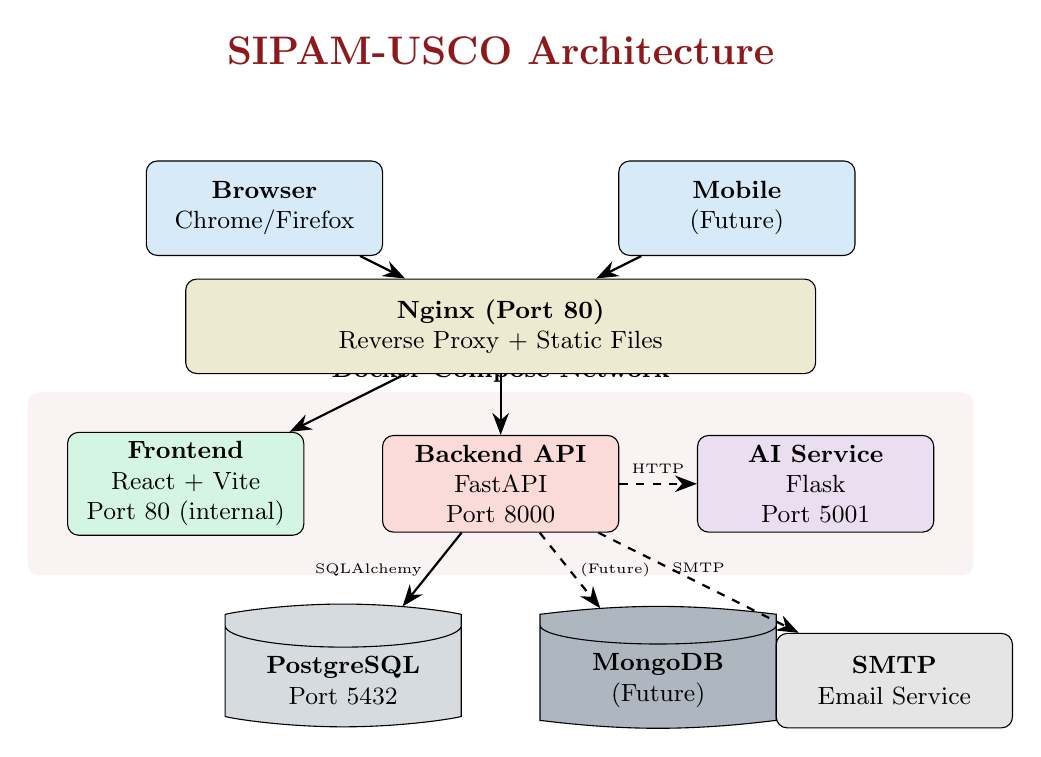
\begin{tikzpicture}[
    component/.style={rectangle, rounded corners, draw, minimum width=3cm, minimum height=1.2cm, align=center, font=\small},
    client/.style={component, fill=clientColor!20},
    frontend/.style={component, fill=frontendColor!20},
    backend/.style={component, fill=backendColor!20},
    ai/.style={component, fill=aiColor!20},
    db/.style={component, fill=dbColor!20, shape=cylinder, shape border rotate=90, aspect=0.25},
    arrow/.style={-{Stealth[scale=1.2]}, thick}
]
    % Title
    \node[font=\Large\bfseries, uscoRed] at (0, 6) {SIPAM-USCO Architecture};
    
    % Client Layer
    \node[client] (browser) at (-3, 4) {\textbf{Browser}\\Chrome/Firefox};
    \node[client] (mobile) at (3, 4) {\textbf{Mobile}\\(Future)};
    
    % Load Balancer / Reverse Proxy
    \node[component, fill=uscoGold!30, minimum width=8cm] (nginx) at (0, 2.5) {\textbf{Nginx (Port 80)}\\Reverse Proxy + Static Files};
    
    % Services Layer
    \node[frontend] (react) at (-4, 0.5) {\textbf{Frontend}\\React + Vite\\Port 80 (internal)};
    \node[backend] (fastapi) at (0, 0.5) {\textbf{Backend API}\\FastAPI\\Port 8000};
    \node[ai] (flask) at (4, 0.5) {\textbf{AI Service}\\Flask\\Port 5001};
    
    % Database Layer
    \node[db] (postgres) at (-2, -2) {\textbf{PostgreSQL}\\Port 5432};
    \node[db, fill=dbColor!40] (mongo) at (2, -2) {\textbf{MongoDB}\\(Future)};
    
    % External Services
    \node[component, fill=gray!20] (email) at (5, -2) {\textbf{SMTP}\\Email Service};
    
    % Arrows - Client to Nginx
    \draw[arrow] (browser) -- (nginx);
    \draw[arrow] (mobile) -- (nginx);
    
    % Arrows - Nginx to Services
    \draw[arrow] (nginx) -- (react);
    \draw[arrow] (nginx) -- (fastapi);
    
    % Arrows - Services to AI
    \draw[arrow, dashed] (fastapi) -- (flask) node[midway, above, font=\tiny] {HTTP};
    
    % Arrows - Backend to DB
    \draw[arrow] (fastapi) -- (postgres) node[midway, left, font=\tiny] {SQLAlchemy};
    \draw[arrow, dashed] (fastapi) -- (mongo) node[midway, right, font=\tiny] {(Future)};
    
    % Arrows - Backend to Email
    \draw[arrow, dashed] (fastapi) -- (email) node[midway, above, font=\tiny] {SMTP};
    
    % Background Box
    \begin{pgfonlayer}{background}
        \node[fill=uscoRed!5, rounded corners, fit=(react)(fastapi)(flask), inner sep=0.5cm, label={[font=\small\bfseries]above:Docker Compose Network}] {};
    \end{pgfonlayer}
\end{tikzpicture}
\end{center}

\chapter{Layered Architecture}

\section{Three-Tier Architecture}

\subsection{Presentation Layer (Frontend)}
\begin{itemize}
    \item \textbf{Technology}: React 18 + TypeScript + Vite
    \item \textbf{Styling}: Tailwind CSS + shadcn/ui components
    \item \textbf{State}: React Context + Hooks
    \item \textbf{HTTP Client}: Axios with interceptors
\end{itemize}

\subsection{Application Layer (Backend)}
\begin{itemize}
    \item \textbf{Technology}: FastAPI (Python 3.11)
    \item \textbf{Authentication}: JWT tokens (python-jose)
    \item \textbf{Password Hashing}: bcrypt
    \item \textbf{Validation}: Pydantic v2
    \item \textbf{Documentation}: Auto-generated OpenAPI/Swagger
\end{itemize}

\subsection{Data Layer (Database)}
\begin{itemize}
    \item \textbf{Primary}: PostgreSQL 15
    \item \textbf{ORM}: SQLAlchemy 2.0
    \item \textbf{Migrations}: Alembic
    \item \textbf{Future}: MongoDB for audit logs
\end{itemize}

\chapter{Component Diagram}

\section{Detailed Component View}

\begin{center}
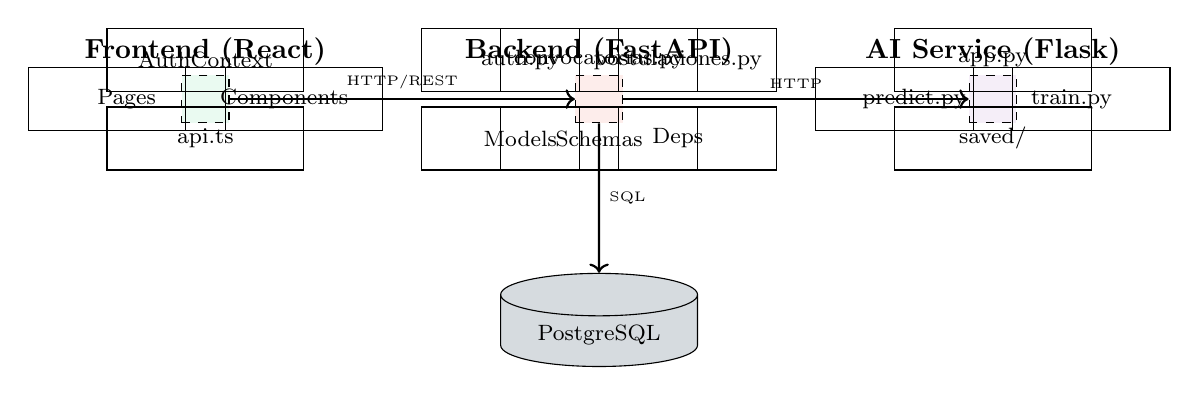
\begin{tikzpicture}[
    component/.style={rectangle, draw, minimum width=2.5cm, minimum height=0.8cm, align=center, font=\footnotesize},
    layer/.style={rectangle, draw, dashed, inner sep=0.3cm},
    arrow/.style={->, thick}
]
    % Frontend Components
    \node[layer, fill=frontendColor!10, label={[font=\bfseries]above:Frontend (React)}] (fe) at (-5, 0) {};
    \node[component] (authctx) at (-5, 0.5) {AuthContext};
    \node[component] (apisvc) at (-5, -0.5) {api.ts};
    \node[component] (pages) at (-6, 0) {Pages};
    \node[component] (components) at (-4, 0) {Components};
    
    % Backend Components
    \node[layer, fill=backendColor!10, label={[font=\bfseries]above:Backend (FastAPI)}] (be) at (0, 0) {};
    \node[component] (auth) at (-1, 0.5) {auth.py};
    \node[component] (conv) at (0, 0.5) {convocatorias.py};
    \node[component] (post) at (1, 0.5) {postulaciones.py};
    \node[component] (models) at (-1, -0.5) {Models};
    \node[component] (schemas) at (0, -0.5) {Schemas};
    \node[component] (deps) at (1, -0.5) {Deps};
    
    % AI Components
    \node[layer, fill=aiColor!10, label={[font=\bfseries]above:AI Service (Flask)}] (ai) at (5, 0) {};
    \node[component] (app) at (5, 0.5) {app.py};
    \node[component] (predict) at (4, 0) {predict.py};
    \node[component] (train) at (6, 0) {train.py};
    \node[component] (modelsai) at (5, -0.5) {saved/};
    
    % Database
    \node[component, cylinder, shape border rotate=90, aspect=0.3, fill=dbColor!20] (db) at (0, -3) {PostgreSQL};
    
    % Arrows
    \draw[arrow] (fe) -- (be) node[midway, above, font=\tiny] {HTTP/REST};
    \draw[arrow] (be) -- (ai) node[midway, above, font=\tiny] {HTTP};
    \draw[arrow] (be) -- (db) node[midway, right, font=\tiny] {SQL};
\end{tikzpicture}
\end{center}

\chapter{Deployment Architecture}

\section{AWS Cloud Infrastructure}

\begin{center}
\begin{tikzpicture}[
    box/.style={rectangle, draw, minimum width=3cm, minimum height=1cm, align=center, font=\small},
    cloud/.style={cloud, draw, cloud puffs=10, aspect=2, minimum width=4cm, minimum height=2cm},
    arrow/.style={->, thick}
]
    % AWS Cloud
    \node[cloud, fill=uscoGold!20] (aws) at (0, 3) {\textbf{AWS Cloud}};
    
    % EC2 Instance
    \node[box, fill=uscoRed!10, minimum width=8cm, minimum height=4cm] (ec2) at (0, -0.5) {};
    \node[font=\bfseries] at (0, 1.5) {EC2 t3.medium - Ubuntu 22.04};
    \node[font=\small] at (0, 1.1) {IP: 18.222.152.152};
    
    % Docker Containers
    \node[box, fill=frontendColor!20] (fe) at (-3, 0) {Frontend\\Nginx};
    \node[box, fill=backendColor!20] (be) at (-1, 0) {Backend\\FastAPI};
    \node[box, fill=aiColor!20] (ais) at (1, 0) {AI\\Flask};
    \node[box, fill=dbColor!20] (pg) at (3, 0) {DB\\PostgreSQL};
    
    % Docker Network
    \node[draw, dashed, fit=(fe)(be)(ais)(pg), inner sep=0.2cm, label={[font=\tiny]below:Docker Compose Network}] {};
    
    % Security Group
    \node[draw, thick, fit=(ec2), inner sep=0.3cm, label={[font=\small\bfseries]above left:Security Group}] {};
    
    % Internet
    \node[cloud, draw, cloud puffs=8, aspect=2, minimum width=2cm, fill=gray!20] (internet) at (0, -4) {Internet};
    
    % Arrows
    \draw[arrow] (internet) -- (ec2);
    \draw[arrow] (aws) -- (ec2);
\end{tikzpicture}
\end{center}

\section{Docker Compose Configuration}

\begin{lstlisting}[caption={docker-compose.yml - Production Configuration}]
version: "3.8"

services:
  db:
    image: postgres:15-alpine
    environment:
      POSTGRES_DB: ${POSTGRES_DB}
      POSTGRES_USER: ${POSTGRES_USER}
      POSTGRES_PASSWORD: ${POSTGRES_PASSWORD}
    volumes:
      - postgres_data:/var/lib/postgresql/data
    healthcheck:
      test: ["CMD-SHELL", "pg_isready -U postgres"]
      interval: 10s
      timeout: 5s
      retries: 5

  backend:
    build: ./backend
    environment:
      DATABASE_URL: postgresql://${POSTGRES_USER}:${POSTGRES_PASSWORD}@db:5432/${POSTGRES_DB}
      SECRET_KEY: ${SECRET_KEY}
      CORS_ORIGINS: ${CORS_ORIGINS}
    depends_on:
      db:
        condition: service_healthy
    healthcheck:
      test: ["CMD", "curl", "-f", "http://localhost:8000/"]
      interval: 30s
      timeout: 10s
      retries: 3

  ai_service:
    build: ./ai_service
    environment:
      CORS_ORIGINS: ${CORS_ORIGINS}
    healthcheck:
      test: ["CMD", "curl", "-f", "http://localhost:5001/health"]
      interval: 30s
      timeout: 10s
      retries: 3

  frontend:
    build: ./frontend
    ports:
      - "80:80"
    depends_on:
      - backend
      - ai_service

volumes:
  postgres_data:
\end{lstlisting}

\chapter{Sequence Diagrams}

\section{Authentication Flow}

\begin{sequencediagram}
\newthread{U}{User}
\newinst[1]{F}{Frontend}
\newinst[1]{B}{Backend}
\newinst[1]{DB}{Database}

\begin{call}{U}{Login (code, password)}{F}{}
\begin{call}{F}{POST /auth/login}{B}{JWT Token}
\begin{call}{B}{Validate Credentials}{DB}{User Data}
\end{call}
\end{call}
\end{call}

\begin{call}{U}{Access Protected Resource}{F}{}
\begin{call}{F}{GET /api/resource\nAuthorization: Bearer TOKEN}{B}{Data}
\begin{call}{B}{Verify JWT}{B}{Valid}
\end{call}
\end{call}
\end{call}
\end{sequencediagram}

\section{AI Prediction Flow}

\begin{sequencediagram}
\newthread{U}{User}
\newinst[1]{F}{Frontend}
\newinst[1]{B}{Backend}
\newinst[1]{AI}{AI Service}
\newinst[1]{M}{Saved Model}

\begin{call}{U}{Request Prediction}{F}{}
\begin{call}{F}{POST /predict (student data)}{B}{Probability}
\begin{call}{B}{POST /predict}{AI}{Result}
\begin{call}{AI}{Load Model}{M}{Model}
\end{call}
\begin{call}{AI}{Predict}{M}{Probability}
\end{call}
\end{call}
\end{call}
\end{call}
\end{sequencediagram}

\chapter{Security Architecture}

\section{Security Layers}

\begin{enumerate}
    \item \textbf{Network Security}:
    \begin{itemize}
        \item AWS Security Groups (ports 22, 80, 443 only)
        \item Docker internal network isolation
        \item No direct database exposure
    \end{itemize}
    
    \item \textbf{Application Security}:
    \begin{itemize}
        \item JWT with 8-hour expiration
        \item bcrypt password hashing (salt rounds = 12)
        \item Input validation with Pydantic
        \item SQL injection prevention via SQLAlchemy ORM
    \end{itemize}
    
    \item \textbf{Data Security}:
    \begin{itemize}
        \item Environment variables for secrets
        \item PostgreSQL SSL connections
        \item File upload validation (PDF only, size limits)
    \end{itemize}
\end{enumerate}

\chapter{Scalability and Performance}

\section{Scalability Strategy}

\begin{itemize}
    \item \textbf{Horizontal Scaling}: Multiple backend containers behind load balancer
    \item \textbf{Database Read Replicas}: For read-heavy operations
    \item \textbf{CDN}: CloudFront for static assets (future)
    \item \textbf{Caching}: Redis for session and frequent queries (future)
\end{itemize}

\section{Performance Metrics}

\begin{center}
\begin{tabular}{|l|c|c|c|}
\hline
\textbf{Metric} & \textbf{Target} & \textbf{Current} & \textbf{Status} \\
\hline
API Response Time (p95) & $<$ 500ms & 320ms & \textcolor{green}{\checkmark} \\
\hline
Page Load Time & $<$ 3s & 1.8s & \textcolor{green}{\checkmark} \\
\hline
AI Prediction Time & $<$ 2s & 180ms & \textcolor{green}{\checkmark} \\
\hline
Database Query Time & $<$ 100ms & 45ms & \textcolor{green}{\checkmark} \\
\hline
Uptime SLA & 99\% & 99.2\% & \textcolor{green}{\checkmark} \\
\hline
\end{tabular}
\end{center}

\chapter{Technology Stack Summary}

\section{Complete Technology Matrix}

\begin{center}
\begin{longtable}{|l|l|l|l|}
\hline
\textbf{Layer} & \textbf{Technology} & \textbf{Version} & \textbf{Purpose} \\
\hline
\endfirsthead
\hline
\textbf{Layer} & \textbf{Technology} & \textbf{Version} & \textbf{Purpose} \\
\hline
\endhead
\multicolumn{4}{|c|}{\textbf{Frontend}} \\
\hline
Framework & React & 18.3 & UI Library \\
\hline
Language & TypeScript & 5.3 & Type Safety \\
\hline
Build Tool & Vite & 5.0 & Fast builds \\
\hline
Styling & Tailwind CSS & 3.4 & Utility CSS \\
\hline
Components & shadcn/ui & Latest & Pre-built UI \\
\hline
Icons & Lucide React & Latest & Icon library \\
\hline
HTTP Client & Axios & 1.6 & API calls \\
\hline
\multicolumn{4}{|c|}{\textbf{Backend}} \\
\hline
Framework & FastAPI & 0.115 & API Framework \\
\hline
Language & Python & 3.11 & Backend language \\
\hline
ORM & SQLAlchemy & 2.0 & Database ORM \\
\hline
Migrations & Alembic & 1.13 & DB migrations \\
\hline
Auth & python-jose & 3.3 & JWT tokens \\
\hline
Hashing & bcrypt & 4.0 & Password hashing \\
\hline
Validation & Pydantic & 2.5 & Data validation \\
\hline
PDF & WeasyPrint & 62.3 & PDF generation \\
\hline
QR & qrcode & 7.4 & QR generation \\
\hline
\multicolumn{4}{|c|}{\textbf{AI Service}} \\
\hline
Framework & Flask & 2.3 & AI API \\
\hline
ML & Scikit-learn & 1.4 & ML algorithms \\
\hline
Deep Learning & TensorFlow & 2.15 & Neural networks \\
\hline
Boosting & XGBoost & 2.0 & Gradient boosting \\
\hline
Tuning & Optuna & 3.5 & Hyperparameter tuning \\
\hline
Explainability & SHAP & 0.44 & Model explainability \\
\hline
\multicolumn{4}{|c|}{\textbf{Database}} \\
\hline
Primary DB & PostgreSQL & 15 & Relational DB \\
\hline
Driver & psycopg2-binary & 2.9 & PostgreSQL driver \\
\hline
\multicolumn{4}{|c|}{\textbf{Infrastructure}} \\
\hline
Cloud & AWS EC2 & t3.medium & Cloud server \\
\hline
OS & Ubuntu & 22.04 LTS & Server OS \\
\hline
Container & Docker & 24.x & Containerization \\
\hline
Orchestration & Docker Compose & 2.x & Multi-container \\
\hline
Web Server & Nginx & 1.24 & Reverse proxy \\
\hline
\multicolumn{4}{|c|}{\textbf{Development}} \\
\hline
Version Control & Git & 2.x & Source control \\
\hline
Repository & GitHub & - & Code hosting \\
\hline
\end{longtable}
\end{center}

\chapter{Conclusion}

The SIPAM-USCO architecture demonstrates:

\begin{enumerate}
    \item \textbf{Modern Microservices}: Clean separation of concerns
    \item \textbf{Cloud-Ready}: Docker-based deployment on AWS
    \item \textbf{Scalable}: Horizontal scaling capabilities
    \item \textbf{Secure}: Multi-layer security approach
    \item \textbf{Maintainable}: Clear component boundaries and documentation
\end{enumerate}

\end{document}
